% !TEX root = ../main.tex
\section{Informativeness-prinsippet}\label{thr:informativeness-principle}

\paragraph{Definisjon.} \emph{Informativeness-prinsippet} (Holmström 1979) sier at et ekstra signal $y$ bør inkluderes i kontrakten hvis og bare hvis det er \emph{statistisk informativt om agentens innsats} $e$ -- dvs.\ at observasjon av $y$ endrer posterior-sannsynligheten for $e$ gitt det primære prestasjonsmålet $Q$. Formelt: $y$ er informativt $\Leftrightarrow$ $f(Q,y|e)$ avhenger av $e$ på en måte som ikke allerede fanges av $Q$ alene. [SLIDE]

\subsection*{Forklaring}

BSZ kap.\ 15 bruker informativeness-prinsippet til å forklare hvorfor kontrakter ofte inkluderer flere måltall, og til å binde sammen (a) kontrollerbarhet, (b) risikodeling, (c) målingers presisjon og (d) risikopremie. [SLIDE/BOK]

\textbf{Kjernelogikk.} I den lineære principal-agent-modellen ($W=W_0+\beta Q$, $Q=\alpha e+\mu$) avhenger den optimale insentivkoeffisienten \thref{incentive-coefficient}{$\beta^*$} av signal-støy-forholdet. Informativeness-prinsippet generaliserer dette: [BOK]

\begin{enumerate}\setlength{\itemsep}{2pt}
\item \textbf{Tilleggssignal $y$.} Anta at et ekstra observerbart signal $y$ er tilgjengelig (f.eks.\ bransjeavkastning, peer-gruppers prestasjon, kundetilfredshet, input-mål).
\item \textbf{Statistisk test.} $y$ er informativt om $e$ $\Leftrightarrow$ fordelingen $f(Q|e,y) \neq f(Q|e)$ for noen $(Q,y)$. Intuitivt: $y$ ``filtrerer bort'' støy fra $Q$ og gjør det lettere å slutte seg til $e$.
\item \textbf{Kontraktuell konsekvens.} Hvis $y$ er informativt, skal optimal kontrakt betinge kompensasjon på \emph{både} $Q$ og $y$: $W = W_0 + \beta_1 Q + \beta_2 y$. Dette \emph{reduserer den effektive støyen} agenten bærer, og tillater høyere $\beta_1$ (sterkere insentiv) uten å øke risikopremien.
\item \textbf{Sufficient statistics.} Omvendt: hvis $Q$ er en \emph{sufficient statistic} for $e$ (all informasjon om $e$ allerede finnes i $Q$), skal $y$ \emph{ikke} inkluderes -- det tilfører bare støy uten innsatsinformasjon.
\end{enumerate}

\textbf{Kobling til de fire delspørsmålene:}

\textbf{(a) Kontrollerbarhet.} \thref{controllability-principle}{Controllability-prinsippet} sier at agenten kun skal måles på det hun kontrollerer. Informativeness-prinsippet \emph{generaliserer} dette: et ukontrollerbart mål kan likevel inkluderes i kontrakten hvis det er informativt om innsats. Eksempel: bransjeavkastning (peer-gruppe) er ikke kontrollerbar av agenten, men er informativ fordi den filtrerer felles markedssjokk fra agentens individuelle prestasjon. [SLIDE]

\textbf{(b) Risikodeling.} Jo mer informative signalene er, desto mer presist kan innsats estimeres, og desto \emph{lavere} risikopremie trenger prinsipalen å betale. Informativeness forbedrer \thref{risk-sharing}{risikodelingen} uten å svekke insentivene. Se formelen: risikopremie $\approx \tfrac{r}{2}\beta^2\sigma^2_{\text{eff}}$ -- informativeness senker $\sigma^2_{\text{eff}}$. [BOK]

\textbf{(c) Målingers presisjon.} Et prestasjonsmål med lav varians $\sigma^2$ er et mer presist signal om innsats. Informativeness-prinsippet predikerer at presise mål bør vektes høyere i kontrakten ($\beta$ høyere), og upresise mål lavere. Mer presise mål $\Rightarrow$ høyere $\beta^*$ $\Rightarrow$ sterkere insentiver $\Rightarrow$ lavere agency costs. [SLIDE]

\textbf{(d) Risikopremie.} Risikopremien $RP = \tfrac{r}{2}\beta^2\sigma^2$ er den direkte kostnaden av å bruke et støyfullt mål som kontraktsgrunnlag. Informativeness-prinsippet sier: legg til signaler som senker effektiv $\sigma^2$, og unngå signaler som bare tilfører støy. Resultatet er lavere $RP$ for gitt insentivnivå. [BOK]

\subsection*{Kjerneforutsetninger}
\begin{itemize}
\item Agentens innsats $e$ er ikke direkte observerbar (\thref{moral-hazard}{moral hazard}).
\item Signaler er kostnadsfritt tilgjengelige (ellers må informasjonsverdien veies mot innsamlingskostnaden).
\item Lineær kontrakt (i generelle modeller gjelder prinsippet mer bredt).
\item Prinsipalen forplikter seg til kontrakten ex ante -- ingen renegotiation.
\end{itemize}

\subsection*{Muligheter}
\begin{itemize}
\item Forklarer hvorfor kontrakter bruker \thref{absolute-vs-relative-performance}{relative prestasjonsmål} (peer-grupper filtrerer felles sjokk).
\item Forklarer indekserte aksjeopsjoner (fjerner markedsbevegelsen, isolerer firmaspesifikk avkastning).
\item Forklarer balansert målekort: flere indikatorer som sammen gir et mer informativt bilde av innsats.
\item Gir normativt kriterium: inkludér et mål $\Leftrightarrow$ det er informativt om innsats.
\item Utvider controllability: ukontrollerbare mål kan likevel være verdifulle.
\end{itemize}

\subsection*{Begrensninger og kritikk}
\begin{itemize}
\item Flere signaler øker kontraktskompleksitet -- agenten forstår kanskje ikke eget insentivsystem (kognitiv overbelastning).
\item Modellen antar at signaler er gratis tilgjengelige -- i praksis koster informasjonsinnsamling.
\item Holmström--Milgrom (1991) multitasking: mer informative mål på én dimensjon kan \emph{vri} innsats bort fra umålbare dimensjoner.
\item Empirisk: vanskelig å teste prinsippet direkte fordi optimal kontraktsdesign er uobserverbar.
\item Forutsetter at regulatoren/prinsipalen kan prosessere mange signaler uten bias -- i praksis brukes tommelfingerregler.
\end{itemize}

\subsection*{Modell / illustrasjon}

\begin{figure}[h]
\centering
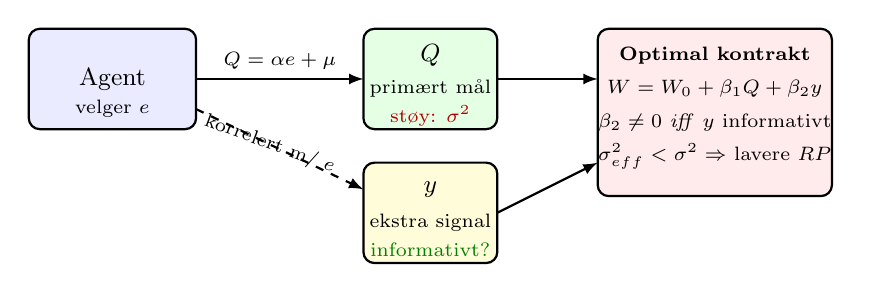
\begin{tikzpicture}[>=latex, scale=0.85, every node/.style={font=\small}]
  % Agent
  \draw[thick, rounded corners, fill=blue!8] (0,2.5) rectangle (2.5,4.0);
  \node at (1.25,3.25) {Agent};
  \node[font=\scriptsize] at (1.25,2.8) {velger $e$};
  % Output Q
  \draw[->, thick] (2.5,3.25) -- (5.0,3.25);
  \node[above, font=\scriptsize] at (3.75,3.25) {$Q = \alpha e + \mu$};
  % Q box
  \draw[thick, rounded corners, fill=green!10] (5.0,2.5) rectangle (7.0,4.0);
  \node at (6.0,3.6) {$Q$};
  \node[font=\scriptsize] at (6.0,3.1) {primært mål};
  \node[font=\scriptsize, red!70!black] at (6.0,2.7) {støy: $\sigma^2$};
  % Extra signal y
  \draw[thick, rounded corners, fill=yellow!15] (5.0,0.5) rectangle (7.0,2.0);
  \node at (6.0,1.6) {$y$};
  \node[font=\scriptsize] at (6.0,1.1) {ekstra signal};
  \node[font=\scriptsize, green!50!black] at (6.0,0.7) {informativt?};
  % Arrow from agent to y
  \draw[->, thick, dashed] (2.5,2.8) -- (5.0,1.6);
  \node[above, font=\scriptsize, rotate=-20] at (3.5,2.0) {korrelert m/ $e$};
  % Contract box
  \draw[thick, rounded corners, fill=red!8] (8.5,1.5) rectangle (12.0,4.0);
  \node[font=\bfseries\scriptsize] at (10.25,3.6) {Optimal kontrakt};
  \node[font=\scriptsize] at (10.25,3.1) {$W = W_0 + \beta_1 Q + \beta_2 y$};
  \node[font=\scriptsize] at (10.25,2.6) {$\beta_2 \neq 0$ \emph{iff} $y$ informativt};
  \node[font=\scriptsize] at (10.25,2.1) {$\sigma^2_{\text{eff}} < \sigma^2 \Rightarrow$ lavere $RP$};
  % Arrows to contract
  \draw[->, thick] (7.0,3.25) -- (8.5,3.25);
  \draw[->, thick] (7.0,1.25) -- (8.5,2.0);
\end{tikzpicture}
\caption{\textbf{Informativeness-prinsippet.} Agenten velger innsats $e$, som påvirker primærmål $Q$ (med støy $\sigma^2$). Et tilleggssignal $y$ inkluderes i kontrakten \emph{bare} hvis det er informativt om $e$ -- altså endrer den statistiske inferensen om $e$ gitt $Q$. Resultat: lavere effektiv støy $\sigma^2_{\text{eff}}$, lavere risikopremie, sterkere insentiver mulig. [SLIDE/BOK]}
\end{figure}

\subsection*{Eksempler}
\begin{itemize}\setlength{\itemsep}{2pt}
\item \textbf{Relative aksjeavkastningsmål (rTSR).} CEO-bonus baseres ikke bare på egen aksjekurs ($Q$) men relativt til peer-gruppe ($y$). Peer-avkastning er informativ om markedssjokk, ikke om CEOs innsats -- ved å trekke fra fjernes felles støy. Informativeness-prinsippet er det teoretiske grunnlaget for rTSR-programmer. [EKS]
\item \textbf{Oljebransjen og oljeprisen.} Oljeprisen er ikke kontrollerbar for Equinor-CEO, men er informativ: den filtrerer ut eksogent prissjokk fra firmaspesifikk prestasjon. Bonus justert for oljepris (eller bransjejustert) bruker informativeness-prinsippet. [EKS]
\item \textbf{Balansert målekort (Kaplan \& Norton).} Finansielle + operasjonelle + kunde + læringsmål: hvert mål tilfører informasjon om dimensjoner av innsats som finansmålet alene ikke fanger -- informativeness-prinsippet begrunner multi-dimensjonell måling. [EKS]
\end{itemize}

\subsection*{Kobling til søyle og andre teorier}
Søyle: \STwo\ (hvilke mål å inkludere) og \SThree\ (kontraktsdesign og $\beta$-valg). Relaterte: \thref{controllability-principle}{Controllability-prinsippet}, \thref{incentive-coefficient}{Incentive coefficient}, \thref{risk-sharing}{Risk sharing}, \thref{optimal-effort-model}{Optimal effort-modell}, \thref{principal-agent}{Principal-agent}, \thref{moral-hazard}{Moral hazard}, \thref{absolute-vs-relative-performance}{Absolutt vs.\ relativ prestasjonsmåling}, \thref{fixed-vs-variable-pay}{Fast vs.\ variabel lønn}, \thref{agency-costs}{Agency costs}.

\paragraph{Brukt i spørsmål:} Q14 (primært), Q09 (referert), Q10 (referert).
